\documentclass[11pt,letterpaper]{article}

%\usepackage{fontspec}
%\usepackage[utf8]{inputenc}
\usepackage{textcomp,marvosym}
\usepackage{amsmath,amssymb}
\usepackage[normalem]{ulem}
\usepackage[left]{lineno}
\usepackage{changepage}
\usepackage{rotating}
\usepackage{color}
\usepackage{natbib}
\usepackage{setspace}
\usepackage{}
\usepackage{fancyhdr}
\usepackage{graphicx}
\usepackage{xspace}
\usepackage{threeparttable}
\usepackage{color,colortbl}
\usepackage{url}
%\usepackage[hidelinks]{hyperref}
\urlstyle{same}
\doublespacing

\raggedright
\textwidth = 6.5 in
\textheight = 8.25 in
\oddsidemargin = 0.0 in
\evensidemargin = 0.0 in
\topmargin = 0.0 in
\headheight = 0.0 in
\headsep = 0.5 in
\parskip = 0.1 in
\parindent = 0.1in

% Bold the 'Figure #' in the caption and separate it from the title/caption with a period
% Captions will be left justified
\usepackage[aboveskip=1pt,labelfont=bf,labelsep=period,justification=raggedright,singlelinecheck=off]{caption}

% Remove brackets from numbering in List of References
%\makeatletter
%\renewcommand{\@biblabel}[1]{\quad#1.}
%\makeatother

% Self defined commands
\newcommand{\degC}{$^{\circ}$C\xspace}
\newcommand{\dC}{$\delta^{13}$C\xspace}
\newcommand{\dO}{$\delta^{18}$O\xspace}
\newcommand{\SrSr}{$^{87}$Sr/$^{86}$Sr\xspace}
\newcommand{\permil}{\textperthousand\xspace}
\newcommand{\dsil}{$d$\xspace}

\setcounter{figure}{0}
\renewcommand{\thefigure}{DR\arabic{figure}}
\setcounter{table}{0}
\renewcommand{\thetable}{DR\arabic{table}}

\definecolor{Yellow}{rgb}{1,1,0.35}
%

\pagestyle{myheadings}
\pagestyle{fancy}
\fancyhf{}
\lhead{Park et al., in review for XXX}
\rhead{\thepage}

\begin{document}

\begin{flushleft}
{\Large \textbf{Data Repository for ``GEOCLIM Modern''}}
\\
Yuem Park\textsuperscript{1},
Nicholas L. Swanson-Hysell\textsuperscript{1},
Pierre Maffre\textsuperscript{2},
Yves Godd\'eris\textsuperscript{2}
\\
\bigskip
\textsuperscript{1} Department of Earth and Planetary Science, University of California, Berkeley, CA, USA
\\
\bigskip

\end{flushleft}

\linenumbers

This document accompanies the discussion contained in the main text. All the Python code used for this study, as well as the associated data tables not included in this document, can be found at: \url{https://github.com/Swanson-Hysell-Group/XXX}.

\section*{Regolith Component}

\begin{figure}[h!]
\begin{center}
	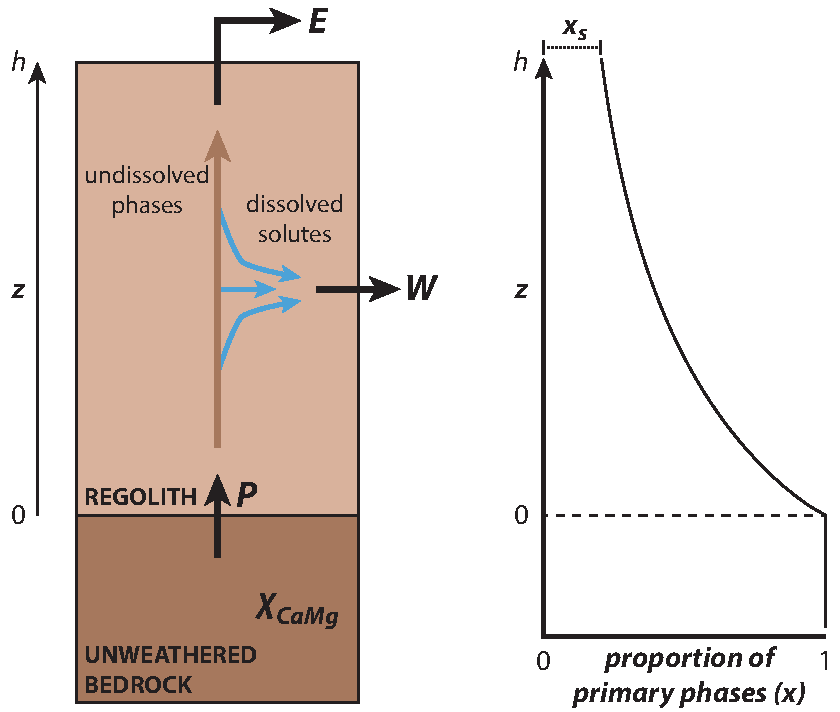
\includegraphics[width=0.5\textwidth]{../Figures/regolith_schematic.pdf}
	\caption{A schematic representation of the regolith component in GEOCLIM at steady state. A rock particle leaves the unweathered bedrock with production rate $P$, and transits vertically through a regolith of height $h$. As the rock particle transits through the regolith, some fraction of the weatherable phases in the rock particle ($x$) are dissolved and leaves the regolith column as weathered phases ($W$). The fraction of the weatherable phases in the rock particle that are not dissolved after transiting through the regolith column leaves it via erosion ($E$).}
	\label{fig:regolith_schematic}
\end{center}
\end{figure}

The regolith component of GEOCLIM models the geochemical evolution of a rock particle as it leaves unweathered bedrock and transits through overlying regolith (Fig. \ref{fig:regolith_schematic}). The component is based upon the theoretical model of \citet{Gabet2009a}, in which material enters the regolith through the downward propagation of the weathering front, and leaves the regolith through physical erosion at the land surface and through the transport of dissolved phases by chemical weathering.

The fundamental processes within the regolith component are described by the following system of three equations:

\begin{equation}
    \frac{dh}{dt} = P - E
    \label{eq:1}
\end{equation}

\begin{equation}
    \frac{\partial x}{\partial t} = -P \frac{\partial x}{\partial z} - K \tau^{\sigma}x
    \label{eq:2}
\end{equation}

\begin{equation}
    \frac{\partial \tau}{\partial t} = -P \frac{\partial \tau}{\partial z} + 1
    \label{eq:3}
\end{equation}

\noindent
Equation \ref{eq:1} is simply a statement of mass conservation, where $h$ is the total height of the regolith (m), $t$ is the time in the model (yr), $P$ is the regolith production rate (m/yr), and $E$ is the physical erosion rate (m/yr). Equation \ref{eq:2} describes how the residual fraction of weatherable phases ($x$, unitless) changes as time in the model ($t$, yr) progresses, where $z$ is the height above the base of the regolith (m). $K \tau^{\sigma}$ is the dissolution rate constant, which depends on the local climate (captured by $K$, yr$^{-1-\sigma}$) and the time that a given rock particle has spent in the regolith ($\tau$, yr) to some power $\sigma$ (unitless). Equation \ref{eq:3} describes how the time that a given rock particle has spent in the regolith changes as time in the model progresses.

The net weathering rate in the regolith column ($W$, m/yr) can then be calculated with:

\begin{equation}
    W = \int_{0}^{h} K \tau^{\sigma} x\;dz
    \label{eq:4}
\end{equation}

The steady state solution of the regolith component is obtained by setting the left hand side of Equations \ref{eq:1}, \ref{eq:2} and \ref{eq:3} to zero.

\citet{Heimsath1997a} found that the rate at which material is entrained into the physically disturbed portion of the regolith (often called soil production) declines exponentially with increasing depth of this disturbed layer. The regolith model that we use does not differentiate the physically disturbed portion of the regolith, but given that the extent of weathering in the regolith below the physically disturbed layer has been found to covary with the rate of soil production \citep{Burke2007a}, we assume that regolith production behaves similarly to soil production:

\begin{equation}
    P = P_{0}\;f(h)
    \label{eq:5}
\end{equation}

\begin{equation}
    P_{0} = k_{rp}\;q\;e^{-\frac{E_{a}}{R}\left(\frac{1}{T}-\frac{1}{T_{0}}\right)}
    \label{eq:6}
\end{equation}

\begin{equation}
    f(h) = e^{-\frac{-h}{d_{0}}}
    \label{eq:7}
\end{equation}

\noindent
$P_{0}$ is the `optimal' regolith production rate (m/yr), which is defined to be the regolith production rate when there is no overlying regolith. In Equation \ref{eq:6}, we parameterize this value using the model of \citet{Carretier2014a}, where $k_{rp}$ is a proportionality constant (unitless), $q$ is the runoff (m/yr), $E_{a}$ is the activation energy (J/K/mol), $R$ is the universal gas constant (J/mol), $T$ is the temperature (K), and $T_{0}$ is the reference temperature (K). $f(h)$ is the `soil production function,' which describes how regolith production decreases as the thickness of the regolith increases. In Equation \ref{eq:7}, we use an exponential equation to represent the soil production function as in \citet{Heimsath1997a}, where $d_{0}$ is a reference regolith thickness (m).

The $K$ in the dissolution rate constant in Equation \ref{eq:2} describes the dependence of the dissolution rate on climate:

\begin{equation}
    K = k_{d}\left(1-e^{-k_{w}q}\right)e^{-\frac{E_{a}}{R}\left(\frac{1}{T}-\frac{1}{T_{0}}\right)}
    \label{eq:8}
\end{equation}

\noindent
Equation \ref{eq:8} is an empirical simplification of mineral dissolution rates derived from kinetic theory and laboratory experiments \citet{West2012a}, where $k_{d}$ is a proportionality constant that modifies the dependence of dissolution rate on runoff and temperature (yr$^{-1-\sigma}$), and $k_{w}$ is a proportionality constant that modified the dependence of dissolution rate on runoff only (yr/m).

Finally, the erosion rate in the regolith component of GEOCLIM uses the parameterization of \citet{Maffre2018a}, which combines the small-scale incision model of \citet{Davy2000a} with the large-scale BQART model of \citet{Syvitski2007a}:

\begin{equation}
    E = k_{e}\;q^{m}\;s^{n}
    \label{eq:9}
\end{equation}

\noindent
$k_{e}$ is a proportionality constant ((m/yr)$^{1-m}$), $s$ is the slope (m/m), and $m$ and $n$ are adjustable exponents.

\section*{Choice of Parameters}

XXX

Experimental determinations of the activation energy (E$_a$) associated with the weathering of silicate minerals are variable \citep{Brantley2003a}. However, multiple efforts to invert for E$_a$ in basaltic watersheds with varying temperature have yielded values (41.6$\pm$3.2 kJ/mol in \citealp{Li2016a}; 42.3 kJ/mol in \citealp{Dessert2001a}) that are consistent with the lower end of activation energies of Ca+Mg bearing minerals in laboratory experiments such as that for diopside (40.5$\pm$1.7 kJ/mol; \citealp{Knauss1993a}) and for labradorite (42.1 kJ/mol; \citealp{Carroll2005a}. We use the values of 42 kJ/mol in our model runs.

\clearpage

\singlespacing

\newpage

\bibliographystyle{gsabull}
\bibliography{References}

\end{document}
